\documentclass[12pt]{article}
\usepackage{graphicx,multicol,mdwlist}
\usepackage{charter,amsmath,amssymb,breakurl}
\usepackage{eulervm}
\usepackage[letterpaper,margin=1in]{geometry}
\title{Math 265 Quiz 4 Warmup Solutions}\author{}\date{}
\let\cos\relax\DeclareMathOperator{\cos}{\mathsf{cos}}
\let\ln\relax\DeclareMathOperator{\ln}{\mathsf{ln}}
\everymath{\displaystyle}
\begin{document}
\maketitle
\thispagestyle{empty}
\begin{multicols}{2}
Questions~\ref{FirstEllipse}--\ref{LastEllipse}
deal with the vector field $\mathbold{F}\left(x,y\right)
=\left\langle x^2-y^2,xy\right\rangle$, which is shown
at the right, together with the curve $C$ consisting of
the top arc of the ellipse $x^2+\frac{y^2}{4}=1$
joined to the line segment from $\left(-1,0\right)$
to $\left(1,0\right)$.
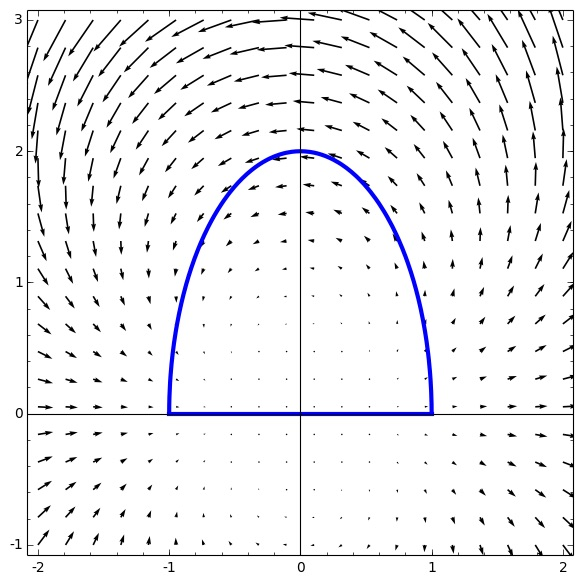
\includegraphics[scale=.4]{Ellipse}
\end{multicols}
\begin{enumerate}
\item\label{FirstEllipse}
Calculate the circulation $\oint_C\mathbold{F}
\cdot d\mathbold{r}$ directly.\\
{\bf Solution.} Parameterize the two parts of the curve
by $\mathbold{r}_1\left(t\right)=\left\langle\cos{t},2\sin{t}\right\rangle$
with $0\le t\le \pi$ and
and $\mathbold{r}_2\left(t\right)=\left\langle t,0\right\rangle$
with $-1\le t\le 1$. The circulation comes out to be $\frac{22}{3}+\frac{2}{3}
=8$.

\item Calculate the circulation $\oint_C\mathbold{F}
\cdot d\mathbold{r}$ using Green's Theorem.\\
{\bf Solution.} We have $Q_x-P_y=3y$ so that
$\int_R3y\;dA=\int_{-1}^1\int_0^{2\sqrt{1-x^2}}3y\;dydx=8$.

\item\label{LastEllipse} Calculate the outward flux $\oint_C\mathbold{F}
\cdot\mathbold{n}\;ds$ using Green's Theorem.\\
{\bf Solution.} We have $P_x+Q_y=3x$ so that
$\int_R3x\;dA=\int_{-1}^1\int_0^{2\sqrt{1-x^2}}3x\;dydx=0$.
Note that the picture above corroborates all of the calculations so far.
\newpage

\suspend{enumerate}
Questions~\ref{FirstConservative}--\ref{LastConservative}
deal with
the vector field $\mathbold{F}\left(x,y,z\right)
=\left\langle 2xy+z^2,x^2,2xz\right\rangle$
and the circle $C$ given by
\[\mathbold{r}\left(t\right)=\left\langle
3\cos{t},4\cos{t},5\sin{t}\right\rangle\]
with $0\le t\le 2\pi$.

\resume{enumerate}
\item\label{FirstConservative} Is $\mathbold{F}$ conservative?\\
{\bf Solution.} We calculate $\mathsf{curl}\left(\mathbold{F}\right)
=\mathbold{0}$, so $\mathbold{F}$ is conservative.
Alternately, the exhibition of a potential function
$f\left(x,y\right)=x^2y+xz^2$ proves that $\mathbold{F}$ is conservative
and obviates the somewhat tedious calculation of
$\mathsf{curl}\left(\mathbold{F}\right)$.

\item Calculate the circulation $\oint_C\mathbold{F}
\cdot d\mathbold{r}$ using a method of your choice.\\
{\bf Solution.} Since $\mathbold{F}$ is conservative
$\oint_C\mathbold{F} \cdot d\mathbold{r}=0$ for {\em any} loop $C$.

\item\label{LastConservative}
Calculate the line integral $\int_D\mathbold{F}
\cdot d\mathbold{r}$ using a method of your choice,
where $D$ is the arc of $C$ with $0\le t\le\frac{\pi}{2}$.\\
{\bf Solution.} Note that $D$ goes from $P=\left(3,4,0\right)$
to $Q=\left(0,0,5\right)$. Using the potential function $f$
calculated in part \ref{FirstConservative} we have
$\int_D\mathbold{F} \cdot d\mathbold{r}=f\left(Q\right)-f\left(P\right)
=-36$.
\end{enumerate}
\end{document}
